\section{WP4 - Crowd plugin development}

\paragraph{Generation of the path}~

\noindent The algorithm of least-effort approach is divided in many points.
\begin{itemize}
  \item Grid arrangement and setting up of the grid.
  \item Computation of the minimum on a graph with the $A*$ algorithm.
  \item Computation of the authorised velocity field.
  \item Finding the exclusion zones in order to do the minisation.
  \item Update of the graph with the attribution of a new weight on the edges: each character affect the weight of its neighbour edges.
\end{itemize}

\noindent We also started coding the classes that we will use (resumed on Figure \ref{crowd_classes}):
\begin{itemize}
  \item Graph: describes the graph that was set up, with a set of nodes and a dictionnary of dictionnaries of edges.
  \item Individual: skeleton rigify, includes position, maximal speed, optimal speed, trajectory and some variable to compute the energy.
  \item Crowd: contains a set of indivuduals and the graph.
  \item Environment: gives the set of forbidden regions.
\end{itemize}

We also try to keep as much code as possible independant from Blender. It will lead to easier tests and a more portable code from Blender to another 3D software.

\begin{figure}[h]
  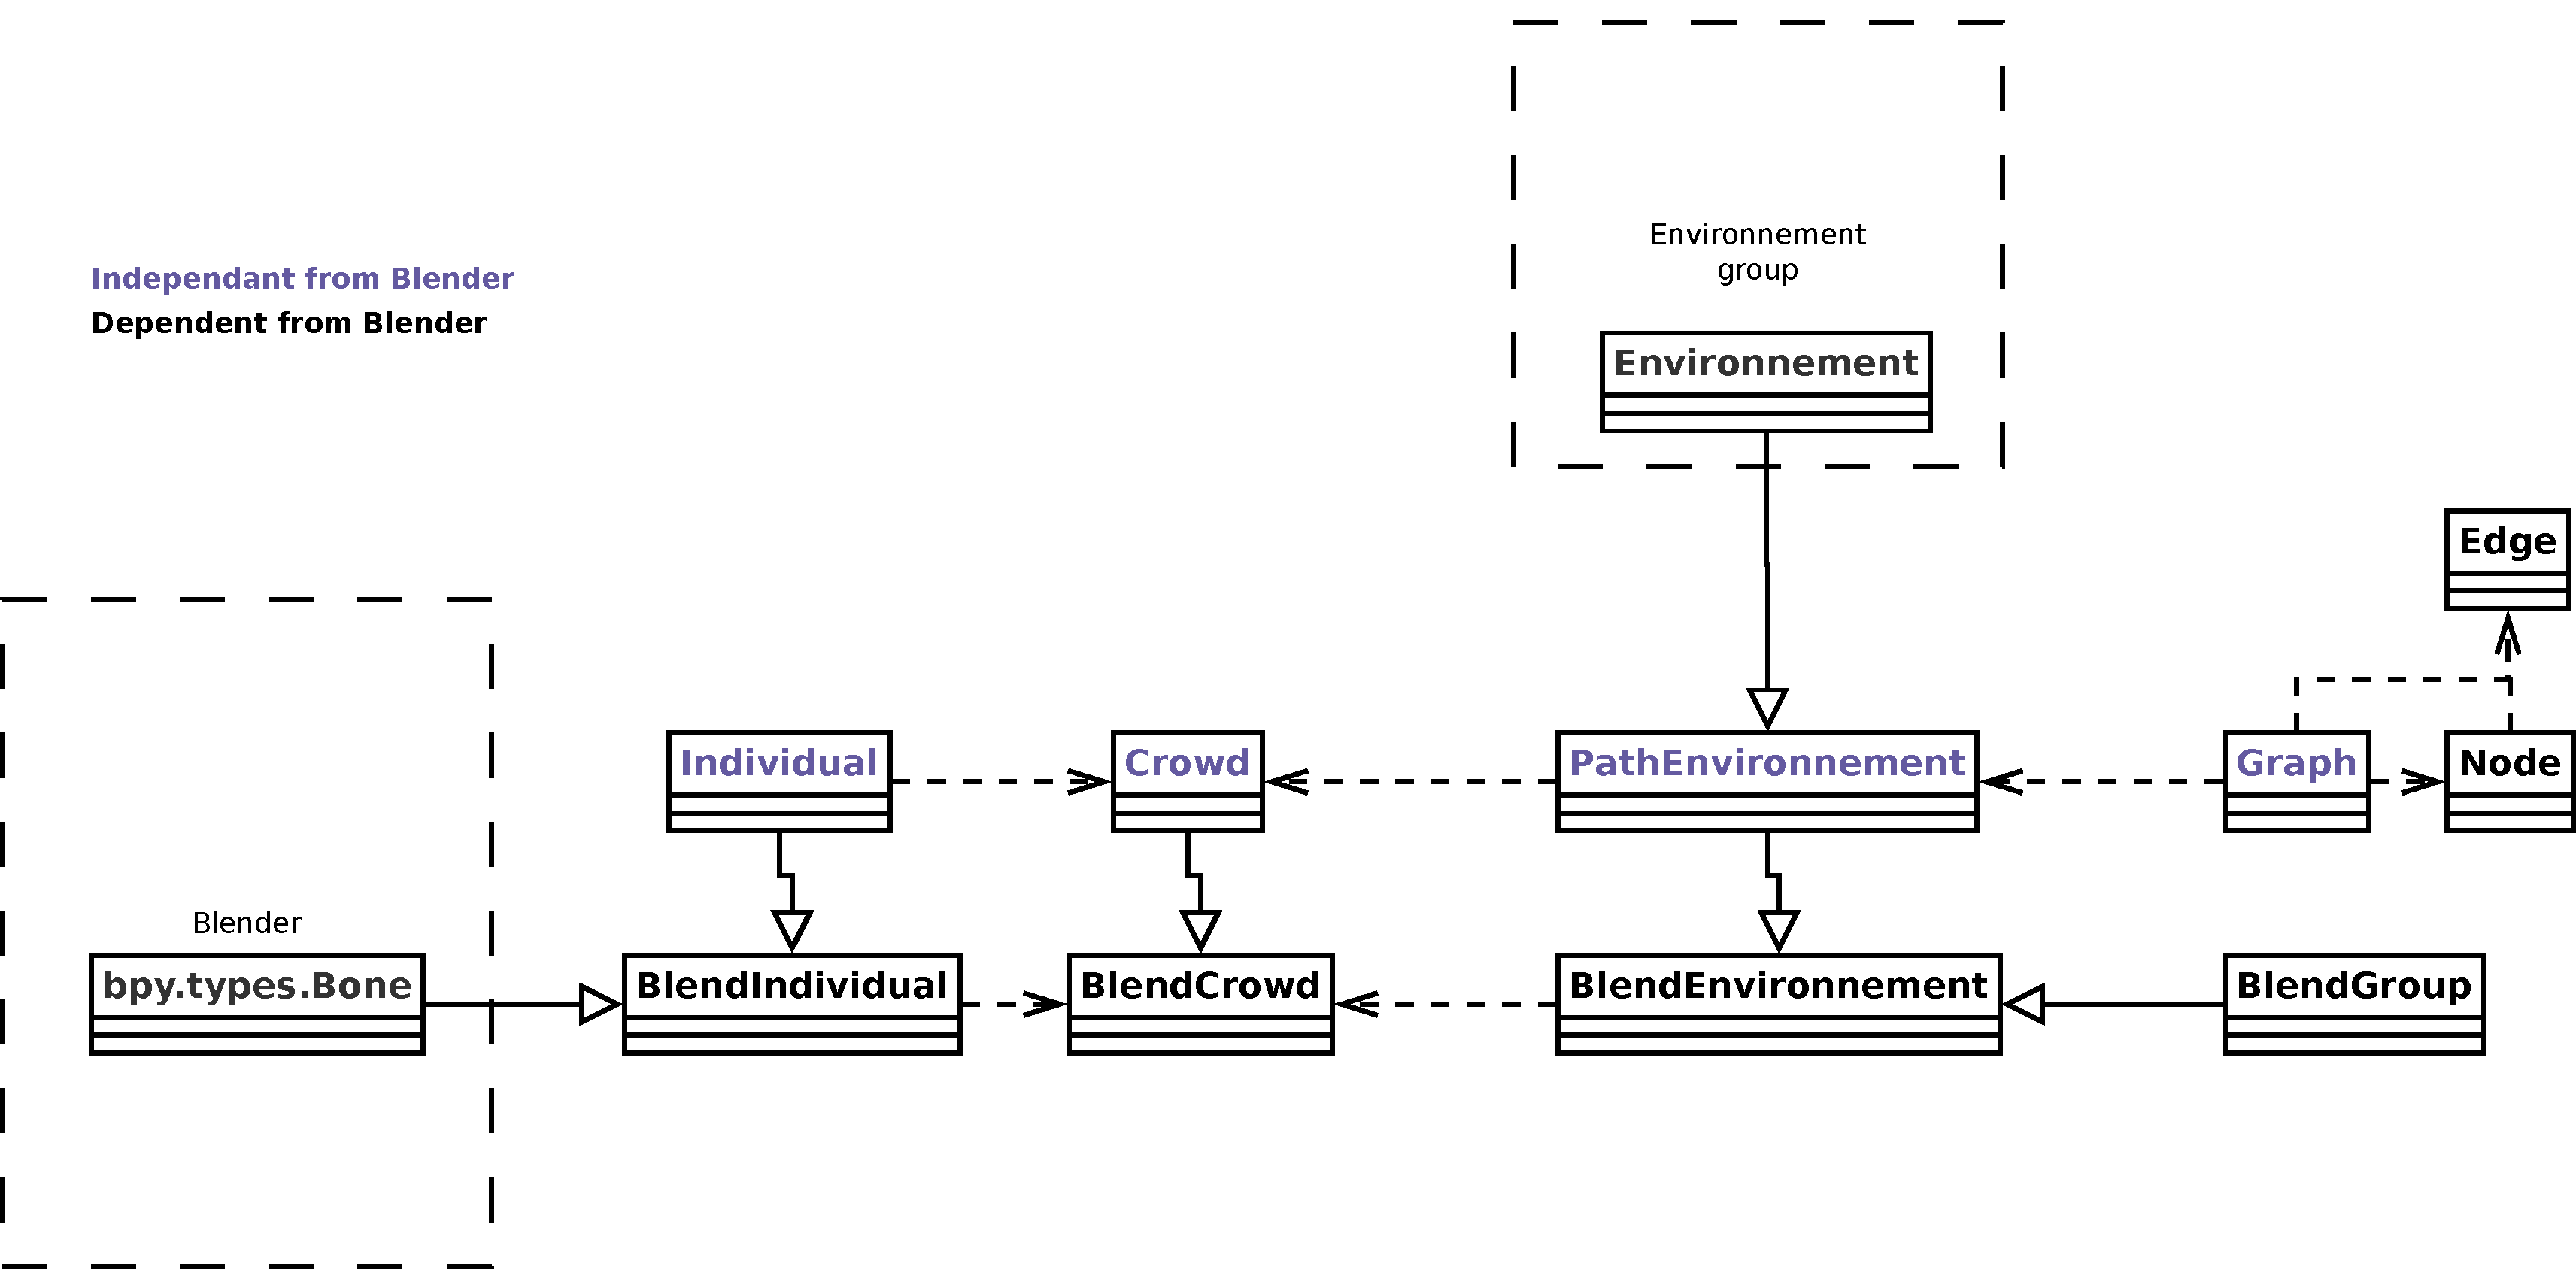
\includegraphics[width=15cm]{crowd_final.pdf}
  \caption{Classes and relations between them.}
  \label{crowd_classes}
\end{figure}

\paragraph{Motions of the characters}~
